\documentclass[]{article}
\usepackage{lmodern}
\usepackage{amssymb,amsmath}
\usepackage{ifxetex,ifluatex}
\usepackage{fixltx2e} % provides \textsubscript
\ifnum 0\ifxetex 1\fi\ifluatex 1\fi=0 % if pdftex
  \usepackage[T1]{fontenc}
  \usepackage[utf8]{inputenc}
\else % if luatex or xelatex
  \ifxetex
    \usepackage{mathspec}
  \else
    \usepackage{fontspec}
  \fi
  \defaultfontfeatures{Ligatures=TeX,Scale=MatchLowercase}
\fi
% use upquote if available, for straight quotes in verbatim environments
\IfFileExists{upquote.sty}{\usepackage{upquote}}{}
% use microtype if available
\IfFileExists{microtype.sty}{%
\usepackage[]{microtype}
\UseMicrotypeSet[protrusion]{basicmath} % disable protrusion for tt fonts
}{}
\PassOptionsToPackage{hyphens}{url} % url is loaded by hyperref
\usepackage[unicode=true]{hyperref}
\hypersetup{
            pdftitle={APLM hw01},
            pdfauthor={san teng},
            pdfborder={0 0 0},
            breaklinks=true}
\urlstyle{same}  % don't use monospace font for urls
\usepackage[margin=1in]{geometry}
\usepackage{color}
\usepackage{fancyvrb}
\newcommand{\VerbBar}{|}
\newcommand{\VERB}{\Verb[commandchars=\\\{\}]}
\DefineVerbatimEnvironment{Highlighting}{Verbatim}{commandchars=\\\{\}}
% Add ',fontsize=\small' for more characters per line
\usepackage{framed}
\definecolor{shadecolor}{RGB}{248,248,248}
\newenvironment{Shaded}{\begin{snugshade}}{\end{snugshade}}
\newcommand{\KeywordTok}[1]{\textcolor[rgb]{0.13,0.29,0.53}{\textbf{#1}}}
\newcommand{\DataTypeTok}[1]{\textcolor[rgb]{0.13,0.29,0.53}{#1}}
\newcommand{\DecValTok}[1]{\textcolor[rgb]{0.00,0.00,0.81}{#1}}
\newcommand{\BaseNTok}[1]{\textcolor[rgb]{0.00,0.00,0.81}{#1}}
\newcommand{\FloatTok}[1]{\textcolor[rgb]{0.00,0.00,0.81}{#1}}
\newcommand{\ConstantTok}[1]{\textcolor[rgb]{0.00,0.00,0.00}{#1}}
\newcommand{\CharTok}[1]{\textcolor[rgb]{0.31,0.60,0.02}{#1}}
\newcommand{\SpecialCharTok}[1]{\textcolor[rgb]{0.00,0.00,0.00}{#1}}
\newcommand{\StringTok}[1]{\textcolor[rgb]{0.31,0.60,0.02}{#1}}
\newcommand{\VerbatimStringTok}[1]{\textcolor[rgb]{0.31,0.60,0.02}{#1}}
\newcommand{\SpecialStringTok}[1]{\textcolor[rgb]{0.31,0.60,0.02}{#1}}
\newcommand{\ImportTok}[1]{#1}
\newcommand{\CommentTok}[1]{\textcolor[rgb]{0.56,0.35,0.01}{\textit{#1}}}
\newcommand{\DocumentationTok}[1]{\textcolor[rgb]{0.56,0.35,0.01}{\textbf{\textit{#1}}}}
\newcommand{\AnnotationTok}[1]{\textcolor[rgb]{0.56,0.35,0.01}{\textbf{\textit{#1}}}}
\newcommand{\CommentVarTok}[1]{\textcolor[rgb]{0.56,0.35,0.01}{\textbf{\textit{#1}}}}
\newcommand{\OtherTok}[1]{\textcolor[rgb]{0.56,0.35,0.01}{#1}}
\newcommand{\FunctionTok}[1]{\textcolor[rgb]{0.00,0.00,0.00}{#1}}
\newcommand{\VariableTok}[1]{\textcolor[rgb]{0.00,0.00,0.00}{#1}}
\newcommand{\ControlFlowTok}[1]{\textcolor[rgb]{0.13,0.29,0.53}{\textbf{#1}}}
\newcommand{\OperatorTok}[1]{\textcolor[rgb]{0.81,0.36,0.00}{\textbf{#1}}}
\newcommand{\BuiltInTok}[1]{#1}
\newcommand{\ExtensionTok}[1]{#1}
\newcommand{\PreprocessorTok}[1]{\textcolor[rgb]{0.56,0.35,0.01}{\textit{#1}}}
\newcommand{\AttributeTok}[1]{\textcolor[rgb]{0.77,0.63,0.00}{#1}}
\newcommand{\RegionMarkerTok}[1]{#1}
\newcommand{\InformationTok}[1]{\textcolor[rgb]{0.56,0.35,0.01}{\textbf{\textit{#1}}}}
\newcommand{\WarningTok}[1]{\textcolor[rgb]{0.56,0.35,0.01}{\textbf{\textit{#1}}}}
\newcommand{\AlertTok}[1]{\textcolor[rgb]{0.94,0.16,0.16}{#1}}
\newcommand{\ErrorTok}[1]{\textcolor[rgb]{0.64,0.00,0.00}{\textbf{#1}}}
\newcommand{\NormalTok}[1]{#1}
\usepackage{graphicx,grffile}
\makeatletter
\def\maxwidth{\ifdim\Gin@nat@width>\linewidth\linewidth\else\Gin@nat@width\fi}
\def\maxheight{\ifdim\Gin@nat@height>\textheight\textheight\else\Gin@nat@height\fi}
\makeatother
% Scale images if necessary, so that they will not overflow the page
% margins by default, and it is still possible to overwrite the defaults
% using explicit options in \includegraphics[width, height, ...]{}
\setkeys{Gin}{width=\maxwidth,height=\maxheight,keepaspectratio}
\IfFileExists{parskip.sty}{%
\usepackage{parskip}
}{% else
\setlength{\parindent}{0pt}
\setlength{\parskip}{6pt plus 2pt minus 1pt}
}
\setlength{\emergencystretch}{3em}  % prevent overfull lines
\providecommand{\tightlist}{%
  \setlength{\itemsep}{0pt}\setlength{\parskip}{0pt}}
\setcounter{secnumdepth}{0}
% Redefines (sub)paragraphs to behave more like sections
\ifx\paragraph\undefined\else
\let\oldparagraph\paragraph
\renewcommand{\paragraph}[1]{\oldparagraph{#1}\mbox{}}
\fi
\ifx\subparagraph\undefined\else
\let\oldsubparagraph\subparagraph
\renewcommand{\subparagraph}[1]{\oldsubparagraph{#1}\mbox{}}
\fi

% set default figure placement to htbp
\makeatletter
\def\fps@figure{htbp}
\makeatother

%\documentclass{article} %虽然加了注释号,但请注意这一行绝对不能注释掉!因为pandoc后生成的tex文件已含有此句
\usepackage[BoldFont,SlantFont,CJKchecksingle]{xeCJK}
\setCJKmainfont[BoldFont=SimSun]{Microsoft YaHei} %我是雅黑控
\setCJKmonofont{SimSun}% 设置缺省中文字体
\parindent 2em   %段首缩进

\title{APLM hw01}
\author{san teng}
\date{2018年10月11日}

\begin{document}
\maketitle

\paragraph{\texorpdfstring{(Programming work) The director of admission
of a small college select 120 students at random from the new freshman
class in a study to determine whether a student's grade point average
(GPA) at the end of freshman year (Y) can be predicted from ACT score
(X). The data information are shown in ''CH01PR19.txt''. Assume X and Y
follows the simple linear regression model with
\(cov(\varepsilon_i , \varepsilon_j ) = 0\) if \(i \neq j\), and
\(cov(\varepsilon_i , \varepsilon_j ) = \sigma^2\) if
\(i = j\).}{(Programming work) The director of admission of a small college select 120 students at random from the new freshman class in a study to determine whether a student's grade point average (GPA) at the end of freshman year (Y) can be predicted from ACT score (X). The data information are shown in ''CH01PR19.txt''. Assume X and Y follows the simple linear regression model with cov(\textbackslash{}varepsilon\_i , \textbackslash{}varepsilon\_j ) = 0 if i \textbackslash{}neq j, and cov(\textbackslash{}varepsilon\_i , \textbackslash{}varepsilon\_j ) = \textbackslash{}sigma\^{}2 if i = j.}}\label{programming-work-the-director-of-admission-of-a-small-college-select-120-students-at-random-from-the-new-freshman-class-in-a-study-to-determine-whether-a-students-grade-point-average-gpa-at-the-end-of-freshman-year-y-can-be-predicted-from-act-score-x.-the-data-information-are-shown-in-ch01pr19.txt.-assume-x-and-y-follows-the-simple-linear-regression-model-with-covvarepsilon_i-varepsilon_j-0-if-i-neq-j-and-covvarepsilon_i-varepsilon_j-sigma2-if-i-j.}

\subsubsection{\texorpdfstring{(a) the least squares estimators
\(\hat{\beta} = (\beta_0 , \beta_1)\)
is:}{(a) the least squares estimators \textbackslash{}hat\{\textbackslash{}beta\} = (\textbackslash{}beta\_0 , \textbackslash{}beta\_1) is:}}\label{a-the-least-squares-estimators-hatbeta-beta_0-beta_1-is}

\begin{Shaded}
\begin{Highlighting}[]
\NormalTok{beta_hat <-}\StringTok{ }\KeywordTok{as.vector}\NormalTok{( }\KeywordTok{solve}\NormalTok{( }\KeywordTok{t}\NormalTok{(X) }\OperatorTok\StringTok{ }\NormalTok{X) }\OperatorTok\StringTok{ }\KeywordTok{t}\NormalTok{(X) }\OperatorTok\StringTok{ }\NormalTok{Y )}
\NormalTok{beta_hat}
\end{Highlighting}
\end{Shaded}

\begin{verbatim}
## [1] 2.11404929 0.03882713
\end{verbatim}

\subsubsection{(b) Plot the fitted regression with
data:}\label{b-plot-the-fitted-regression-with-data}

\begin{Shaded}
\begin{Highlighting}[]
\NormalTok{g <-}\StringTok{ }\KeywordTok{ggplot}\NormalTok{(data, }\KeywordTok{aes}\NormalTok{(}\DataTypeTok{x =}\NormalTok{ Score, }\DataTypeTok{y =}\NormalTok{ GPA)) }\OperatorTok{+}\StringTok{ }\KeywordTok{geom_point}\NormalTok{() }
\NormalTok{g }\OperatorTok{+}\StringTok{ }\KeywordTok{geom_abline}\NormalTok{(}\DataTypeTok{intercept =}\NormalTok{ beta_hat[}\DecValTok{1}\NormalTok{] ,}\DataTypeTok{slope =}\NormalTok{ beta_hat[}\DecValTok{2}\NormalTok{])}
\end{Highlighting}
\end{Shaded}

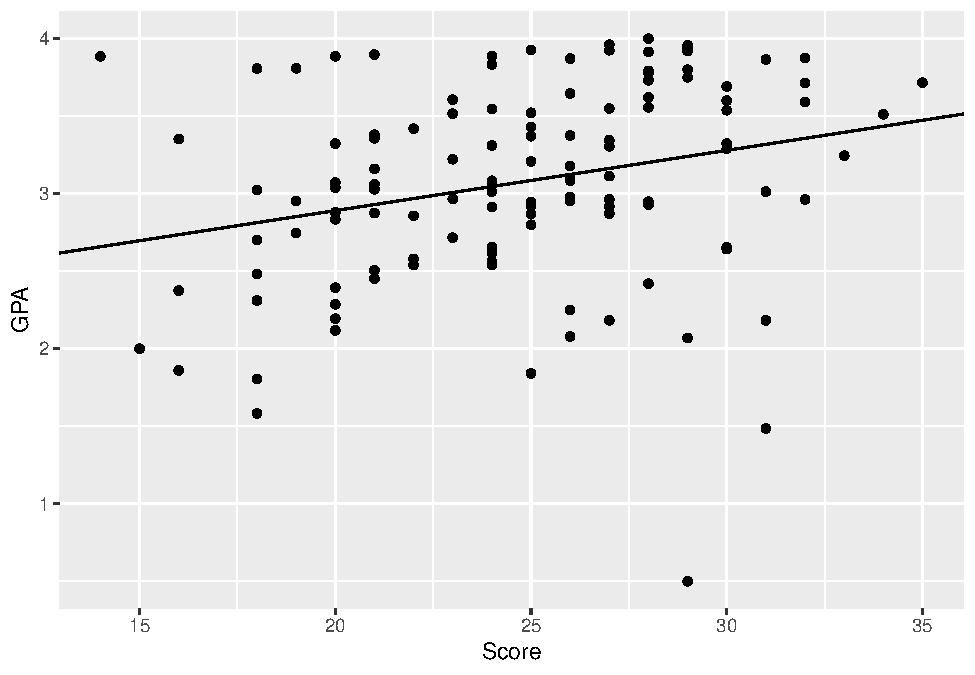
\includegraphics{APLM-hw01_files/figure-latex/(b)Plot-1.pdf}

\subsubsection{我認為這條線(fitted
line)並沒有對Score和GPA作出明顯的趨勢呈現。}\label{ux6211ux8a8dux70baux9019ux689dux7ddafitted-lineux4e26ux6c92ux6709ux5c0dscoreux548cgpaux4f5cux51faux660eux986fux7684ux8da8ux52e2ux5448ux73fe}

\subsubsection{Score 和
GPA並沒有到很明顯的正比關係。在Score介於25\textasciitilde{}30間,有一些點是GPA低的點,使得如果不看這些資料點,則有著Score愈高,GPA愈高的趨勢。}\label{score-ux548c-gpaux4e26ux6c92ux6709ux5230ux5f88ux660eux986fux7684ux6b63ux6bd4ux95dcux4fc2ux5728scoreux4ecbux65bc2530ux9593ux6709ux4e00ux4e9bux9edeux662fgpaux4f4eux7684ux9edeux4f7fux5f97ux5982ux679cux4e0dux770bux9019ux4e9bux8cc7ux6599ux9edeux5247ux6709ux8457scoreux6108ux9ad8gpaux6108ux9ad8ux7684ux8da8ux52e2}

\subsubsection{(c) the residuals and sum of residuals
is:}\label{c-the-residuals-and-sum-of-residuals-is}

\begin{Shaded}
\begin{Highlighting}[]
\NormalTok{residual <-}\StringTok{ }\NormalTok{Y }\OperatorTok{-}\StringTok{ }\NormalTok{X }\OperatorTok\StringTok{ }\NormalTok{beta_hat}
\NormalTok{sum_of_residual <-}\StringTok{ }\KeywordTok{sum}\NormalTok{(residual}\OperatorTok{^}\DecValTok{2}\NormalTok{)}
\KeywordTok{head}\NormalTok{(residual)}
\end{Highlighting}
\end{Shaded}

\begin{verbatim}
##             [,1]
## [1,]  0.96758105
## [2,]  1.22737094
## [3,]  0.57679116
## [4,] -0.42824608
## [5,]  0.09858105
## [6,]  0.54730978
\end{verbatim}

\begin{Shaded}
\begin{Highlighting}[]
\NormalTok{sum_of_residual}
\end{Highlighting}
\end{Shaded}

\begin{verbatim}
## [1] 45.81761
\end{verbatim}

\subsubsection{\texorpdfstring{(d) Estimate \(\sigma^2\) and \(\sigma\)
by MSE and
\(\sqrt{MSE}\):}{(d) Estimate \textbackslash{}sigma\^{}2 and \textbackslash{}sigma by MSE and \textbackslash{}sqrt\{MSE\}:}}\label{d-estimate-sigma2-and-sigma-by-mse-and-sqrtmse}

\begin{Shaded}
\begin{Highlighting}[]
\NormalTok{MSE <-}\StringTok{ }\NormalTok{sum_of_residual }\OperatorTok{/}\StringTok{ }\NormalTok{(}\KeywordTok{dim}\NormalTok{(data)[}\DecValTok{1}\NormalTok{] }\OperatorTok{-}\StringTok{ }\DecValTok{2}\NormalTok{)}
\NormalTok{MSE}
\end{Highlighting}
\end{Shaded}

\begin{verbatim}
## [1] 0.3882848
\end{verbatim}

\begin{Shaded}
\begin{Highlighting}[]
\KeywordTok{sqrt}\NormalTok{(MSE)}
\end{Highlighting}
\end{Shaded}

\begin{verbatim}
## [1] 0.623125
\end{verbatim}

\end{document}
